\documentclass[UTF8, a4paper, linespread=1.5]{article}

\usepackage{tcolorbox, listings, algorithm, minted, algpseudocode}
\usepackage{geometry, savesym, amsmath, enumerate, indentfirst, color, amsthm, bm, extarrows, ulem}
\usepackage{amssymb}
\usepackage{nameref, hyperref}
 \geometry{top=3cm, bottom=3cm, left=1.5cm, right=1.5cm}

\usepackage{enumitem}
\setenumerate[1]{itemsep=0pt,partopsep=0pt,parsep=\parskip,topsep=5pt}
\setitemize[1]{itemsep=0pt,partopsep=0pt,parsep=\parskip,topsep=5pt}

\renewcommand\contentsname{Contents}

\tcbuselibrary{skins, breakable, theorems}

% \setlength{\leftskip}{10pt}
\setlength{\parindent}{10pt}
% \setlength{\parskip}{2em}
\renewcommand{\baselinestretch}{1.3}

\newcounter{RomanNumber}
\newcommand{\mrm}[1]{(\setcounter{RomanNumber}{#1}\Roman{RomanNumber})}

\newtcbtheorem{thm}{}
  {enhanced, theorem name and number, code={\edef\@currentlabelname{#2}}, 
  frame code={
        % \path[thick, draw] (frame.north west) -| (frame.north east) -| (frame.south east) -| (frame.south west) -| (frame.north west);
        \path[thick, draw] (frame.north west)  +(.5\baselineskip,0) -| +(0,-.5\baselineskip);
        % \path[thick, draw] (frame.north east) +(-.5\baselineskip,0) -| +(0,-.5\baselineskip);
        % \path[thick, draw] (frame.south west) +(.5\baselineskip,0) -| +(0,.5\baselineskip);
        \path[thick, draw] (frame.south east) +(-.5\baselineskip,0) -| +(0,.5\baselineskip);
    },
    left=1mm, right=1mm, top=1mm, bottom=1mm,
    colback=black!5,
    colframe=red!75!black,
    colbacktitle=black!0,
    coltitle=black!100,
    fonttitle=\bfseries}{thm}


\usepackage{environ}
\RenewEnviron{math}{%
\begin{align*}
\BODY
\end{align*}
}

\title{CS217 -- Algorithm Design and Analysis \\ Homework 5}
\date{\today}
\author{Not Strong Enough}



\begin{document}

    \maketitle

    \begin{thm}{}{}
        Let $v(G)$ denote the size of a maximum matching of $G$.
        Obviously, $val(MLP(G))\ge v(G)$ for all graphs.
        Show that $v(G)=val(MLP(G))$ for all bipartite graphs $G$.
        Do this without referring to Konig's Theorem.
    \end{thm}
    \begin{proof}[Solution]
        Suppose $X$ is a solution to $MLP(G)$.
        $E_F$ is the set of edges with fractional values in X.
        First do as follows:
        \begin{itemize}
            \item[(1)] If $E_F$ doesn't contain a cycle, terminate.
            \item[(2)] Find a cycle in $E_F$ with fractional values, denote it $C:=\{e_i\in E_F :1\le i \le n,i\in\mathbb{N}\}$.
            \item[(3)] Add $x_{e_{2k-1}}$ by $\epsilon$ and $x_{e_{2k}}$ by $-\epsilon$ for $\{k\in \mathbb{N}:k<=n/2\}$.
            \item[(4)] Increase $\epsilon$ until there exists $i$ such that $x_{e_i}=0 \text{ or } 1$.
            \item[(5)] go to step(2) if there exists a cycle in $E_F$.
        \end{itemize}
        Since $G$ is a bipartite, C can only be a even cycle, so step (3) makes sense.
        If we modify the solution by step(3) , obviously the constraints of $MLP(G)$ will still be satisfied, and the target function will remain unchanged.
        The process will terminate because $|E_F|$ decreases by at least 1 in each iteration.

        Then do as follows:
        \begin{itemize}
            \item[(1)] If $E_F$ is empty, terminate.
            \item[(2)] Choose 2 vertex $v_1,v_2$ that $|\{x_e\in(0,1):v_1\in e\}|=1$, $|\{x_e\in(0,1):v_2\in e\}|=1$ and there's a path between $v_1$ and $v_2$ in $E_F$, denote it $P:=\{e_{i}'\in E_F:1\le i \le m,i\in\mathbb{N}\}$
            \item[(3)] Add $x_{e_{2k-1}'}$ by $\epsilon$ for $\{k\in\mathbb{N}:2k-1\le m\}$ and $x_{e_{2k}'}$ by $-\epsilon$ for $\{k\in\mathbb{N}:2k\le m\}$
            \item[(4)] Increase $\epsilon$ until there exists $i$ such that $x_{e_{i}'}=0 \text{ or } 1$
            \item[(5)] Go to step (2) if $E_F$ is not empty
        \end{itemize}
        Since there's no cycle in $E_F$, we can definitely choose $v_1,v_2$ that satisfy the requirements if $E_F$ is not empty.
        In each iteration, the target function will not decrease.
        Since $v_1,v_2$ can only be touched by edges with fractional value or value 0, the constraints of $v_1,v_2$ can be satisfied.
        In other words, $\sum_{e\in E:v_1\in e}x_e =x_{e_{1}'} \le 1$, $\sum_{e\in E:v_2\in e}x_e =x_{e_{m}'} \le 1$
        The constraints of other vertices $v$ in $P$ will obviously be maintained.
        The process will termintate because $|E_F|$ decreases by at least 1 in each iteration.

        Finally, after 2 processes, the solution becomes integral and the value of target function does not decrease, which means $\text{int-val}(MLP(G))\ge val(MLP(G))$.
        However we have  $\text{int-val}(MLP(G))\le val(MLP(G))$.
        So $v(G)=\text{int-val}(MLP(G))= val(MLP(G))$
    \end{proof}


    \begin{thm}{}{}
        We know that $\nu(G) = \tau(G)$ for all bipartite graphs (K\H{o}nig's Theorem) and $\nu(G) \leq \tau(G)$ for all graphs (since every matched edge must be covered by a distinct vertex). Show that $\tau(G) \leq 2\nu(G)$ for all grpahs $G$.
    \end{thm}

    \begin{proof}
        Let $M$ be a maximum matching of $G$. It follows that $|M| = \nu(G)$. Now we choose our vertex set $V'$ to be all the matched vertices in $G$. So $|V'| = 2\nu(G)$. 
        
        Claim that $V'$ is a vertex cover. To see that, assume there exists an edge $(u, v)$ which is not covered by $V'$. It means that neither $u$ nor $v$ is matched. So we can add edge $(u, v)$ to $M$, and thus $M$ is not maximum, which leads to a contradiction.
        
        So the size of minimum vertex cover $\tau(G) \leq |V'| = 2\nu(G)$.
    \end{proof}

    \begin{thm}{}{}
        Show that $\tau(G) \leq 2{\rm opt}({\rm VCLP}(G))$ for all graphs $G$ (including non-bipartite graphs).
    \end{thm}

    \begin{proof}
        From (2) we know that $\tau(G) \leq 2\nu(G)$. Since $\nu(G) \leq {\rm opt}({\rm MLP}(G)) \leq {\rm opt}({\rm VCLP}(G))$, it follows that $\tau(G) \leq 2\nu(G) \leq 2{\rm opt}({\rm VCLP}(G))$.
    \end{proof}

    \begin{thm}{}{}
        For a graph $G = (V, E)$, let $\tau(G)$ denote the size of a minimum vertex cover, and $\nu(G)$ the size of a maximum matching. Recall the two linear programs VCLP and MLP. Let $\tau_f(G) := {\rm opt}({\rm VCLP}(G))$ and $\nu_f(G) := {\rm opt}({\rm MLP}(G))$. Note that
        $$
        \nu(G) \leq \nu_f(G) = \tau_f(G) \leq \tau(G),
        $$
        where the equality in the middle follows from Strong LP Duality. Also, if $G$ is bipartite, then the equality holds throughout in (1). Let us say a graph $G$ is {\it VCLP exact} if $\tau(G) = \tau_f(G)$, and {\it MLP exact} if $\nu(G) = \nu_f(G)$. As we already know, a bipartite grpah $G$ is both VCLP exact and MLP exact.
        
        From now on, suppose that $G$ is {\it not} bipartite but $\tau(G) = \tau_f(G)$.
        
        \begin{enumerate}
            \item Give an example of such a graph $G$ that is not bipartite but still VCLP exact.
            \item Give an example of a graph $G$ that is MLP exact but not VCLP exact.
            \item Suppose $G$ is VCLP exact. Let $Y \subseteq V(G)$ be a minimum vertex cover. Let $\mathbf{x}$ be an optimal solution of MLP($G$). Show that $x_e = 0$ if $e \subseteq Y$ (i.e., if both endpoints of $e$ are in the cover).
            \item Show that such a graph $G$ has a matching of size $|Y|$, and thus is MLP exact, too.
        \end{enumerate}
    \end{thm}

    \begin{center}
        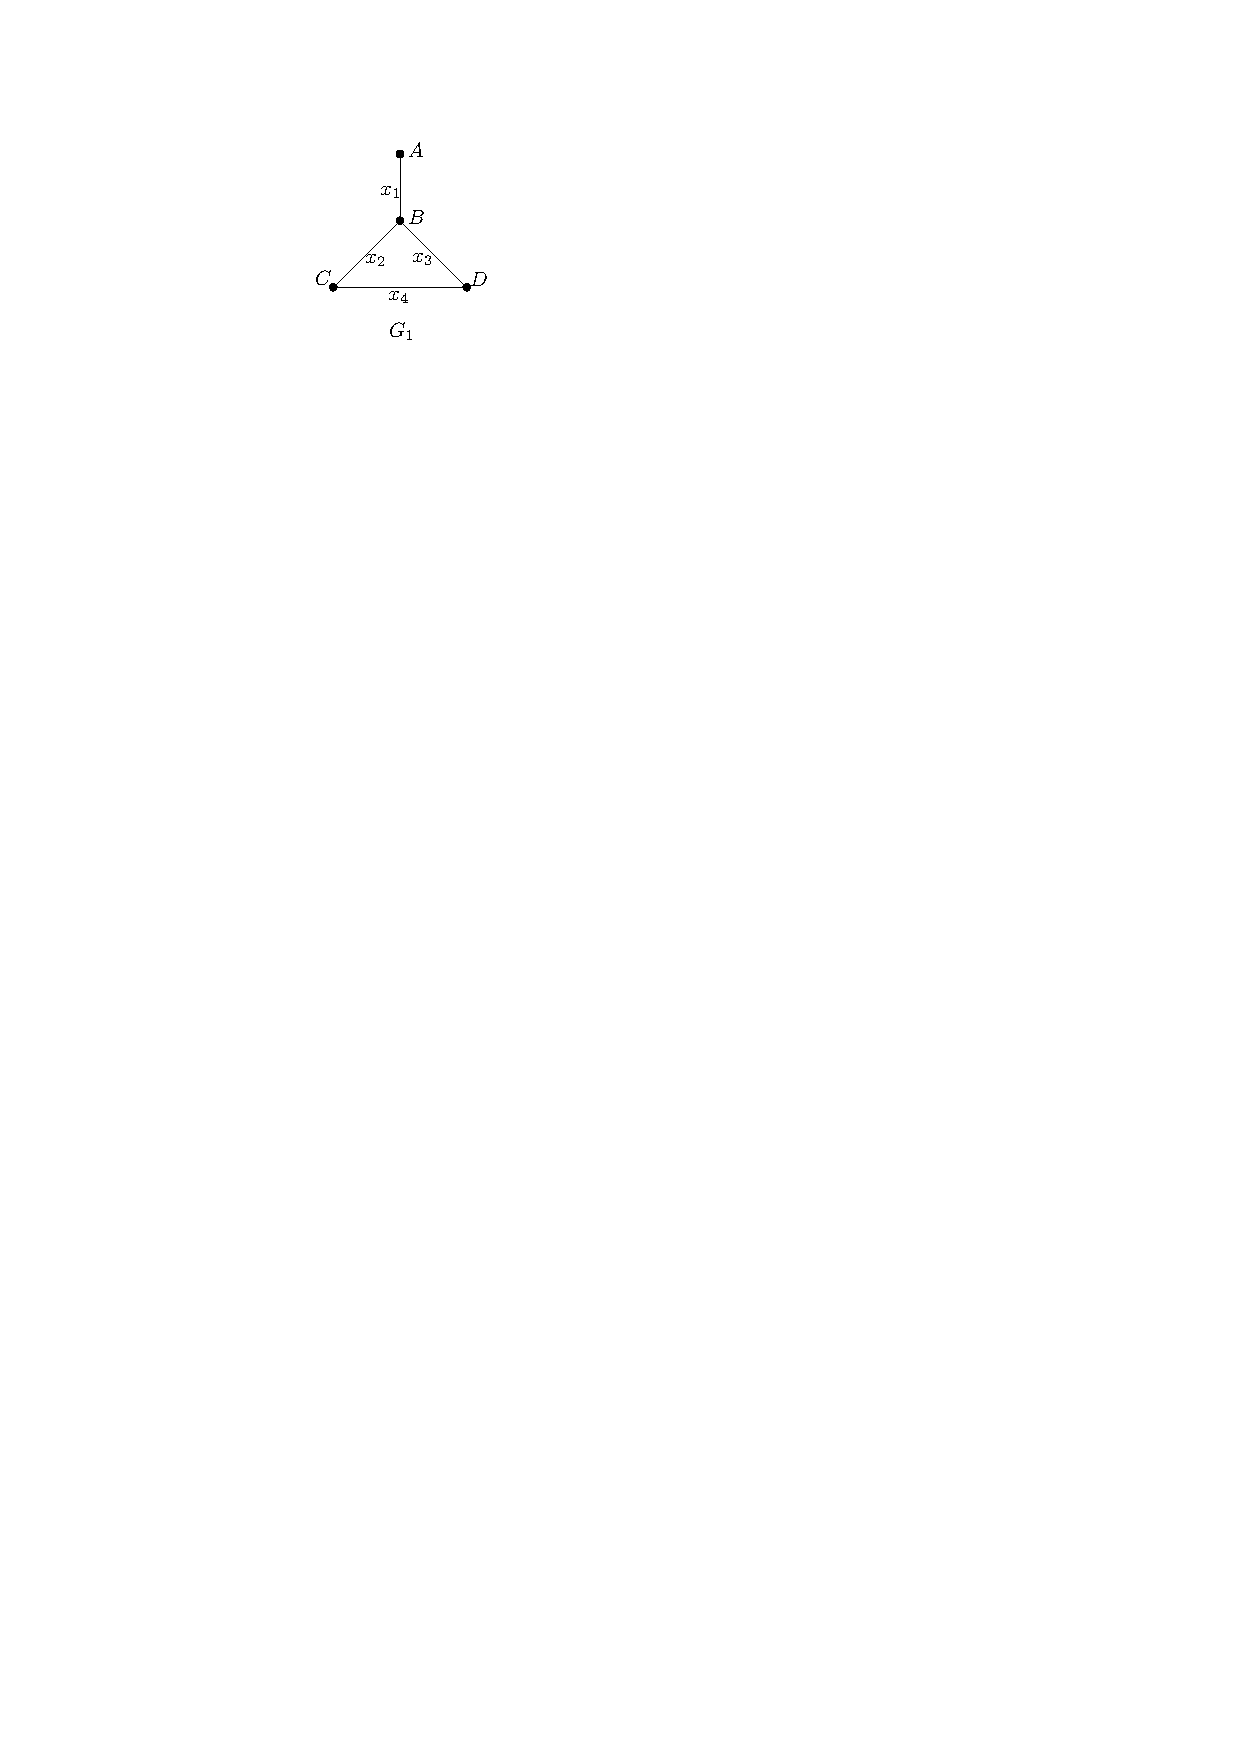
\includegraphics[width=0.16\textwidth]{figure4_1.pdf}
        \hspace{3cm}
        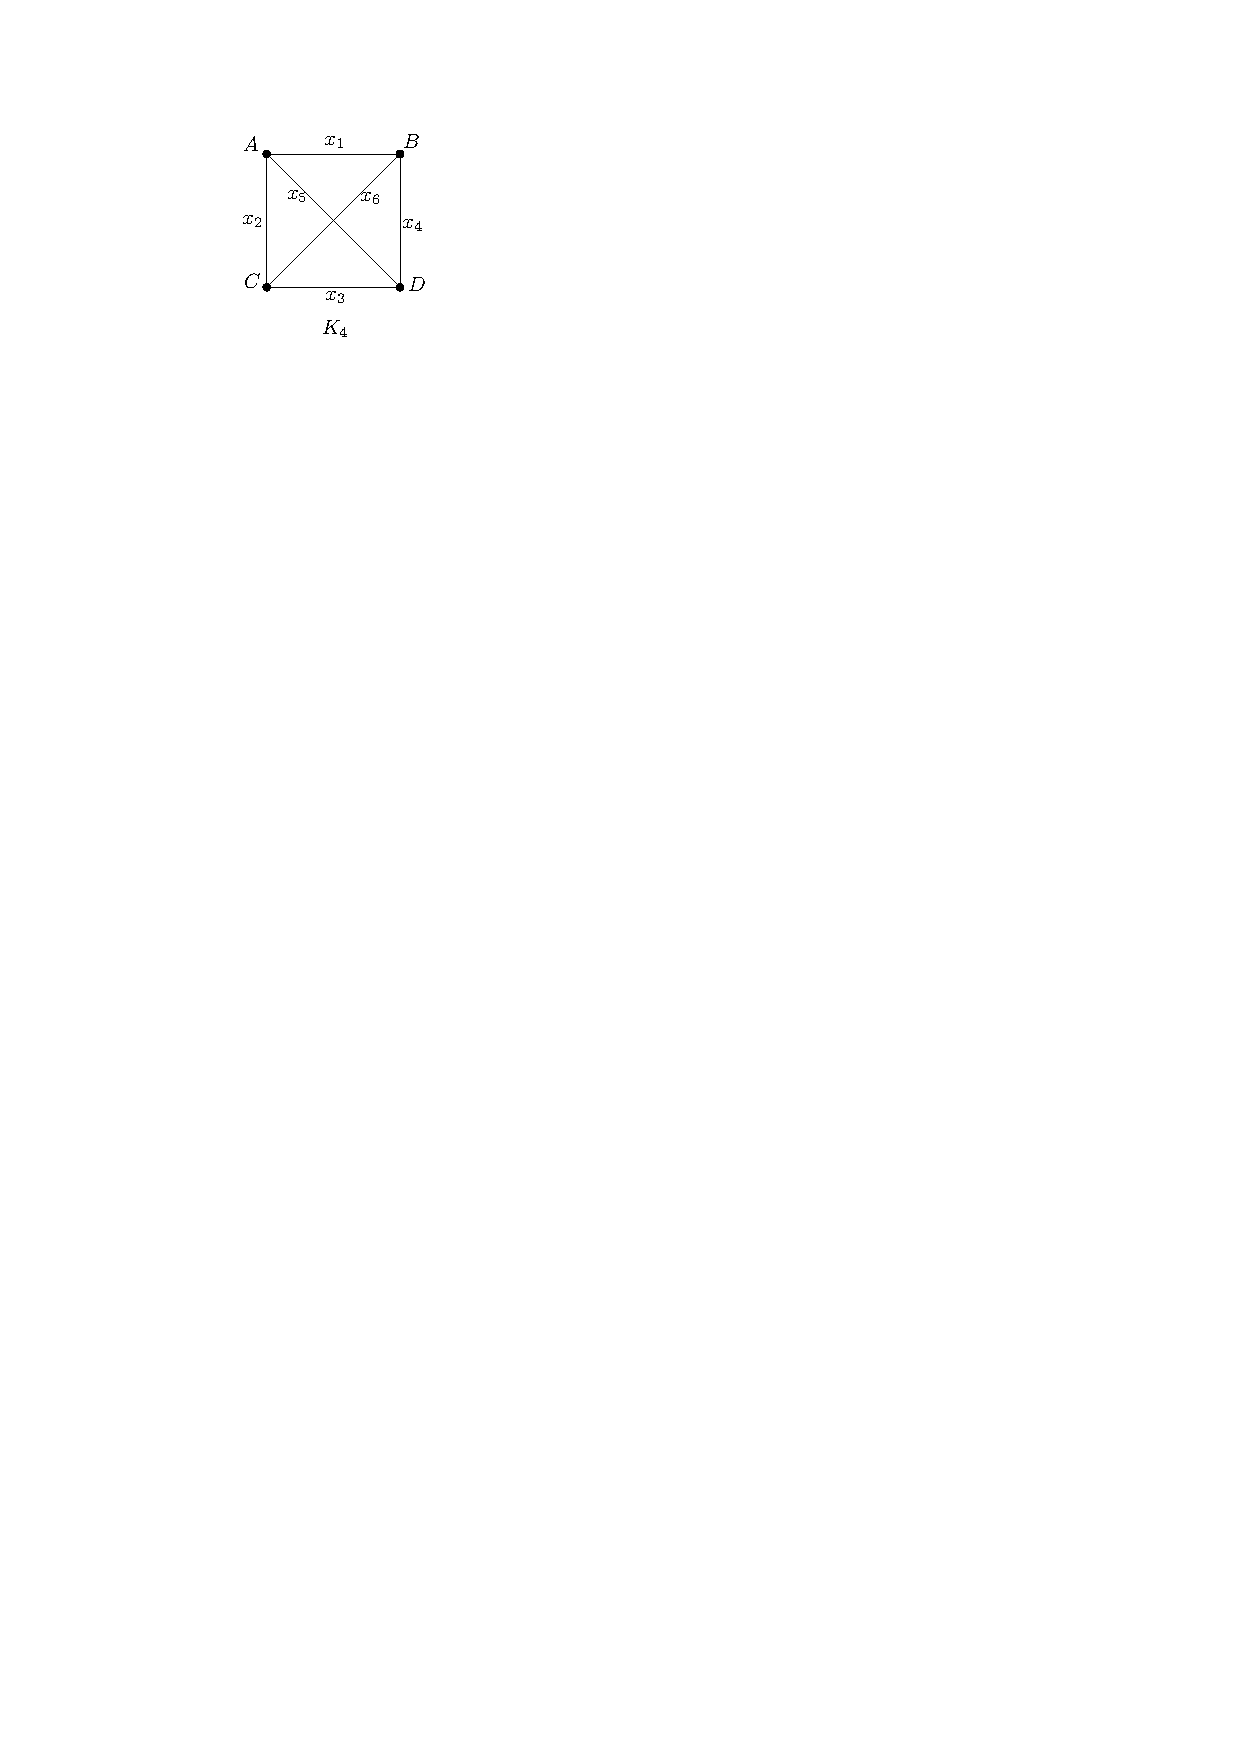
\includegraphics[width=0.16\textwidth]{figure4_2.pdf}
    \end{center}

    \begin{proof}[Solution.]
        ~
        \begin{enumerate}
            \item The example is $G_1$ in the upper left. It is not bipartite since $B, C, D$ constitute an odd cycle.
            
            The minimum vertex cover of $G_1$ can be $\{B, C\}$ or $\{B, D\}$, with size $2$. So $\tau(G_1) = 2$.
            
            VCLP$(G_1)$ is
            \begin{center}
                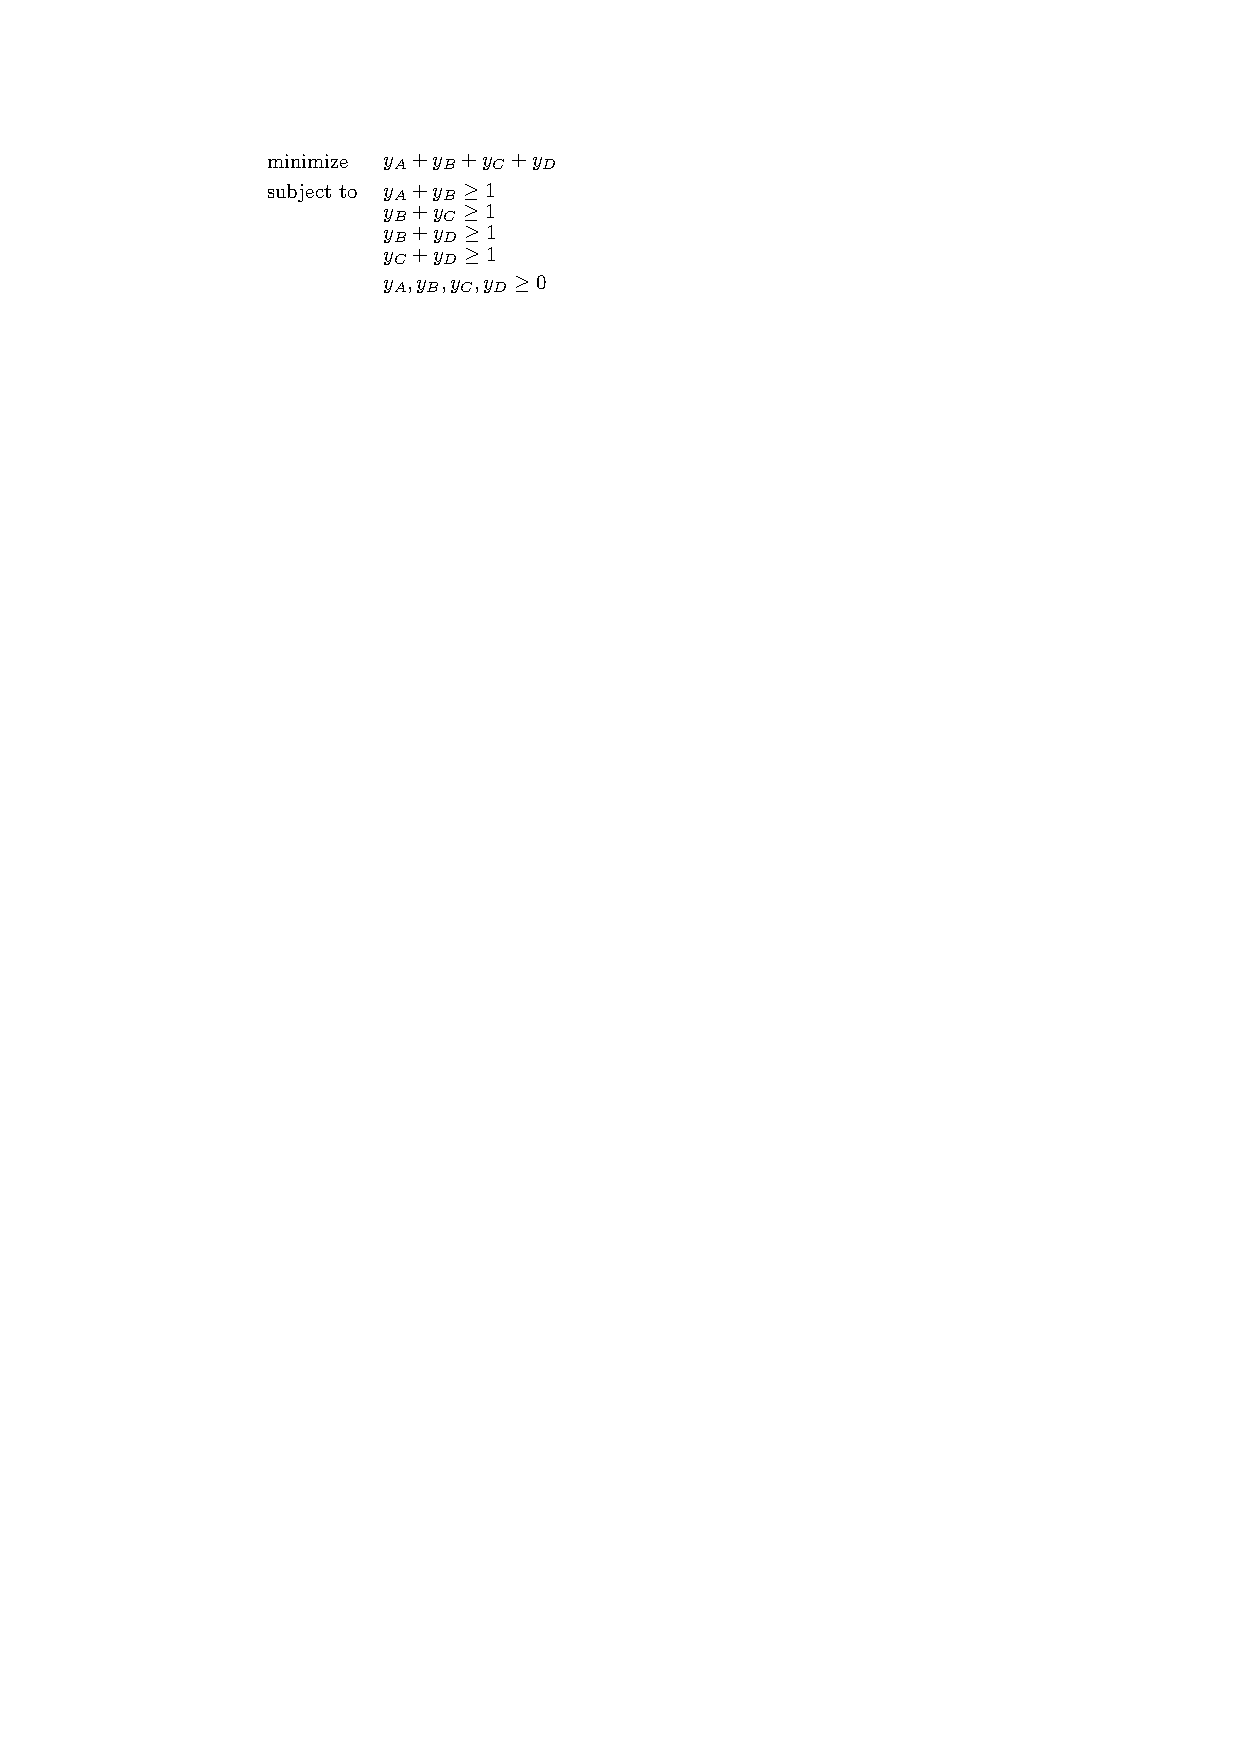
\includegraphics[width=0.28\textwidth]{VCLP4_1.pdf}
            \end{center}
            Note that if we add up the constraints $y_A + y_B \geq 1$ and $y_C + y_D \geq 1$, we get $y_A + y_B + y_C + y_D \geq 2$, which gives a lower bound of the target function.
            
            Since $\tau(G_1) = 2$, it follows that the lower bound is tight. Hence $\tau_f(G_1) = \tau(G_1) = 2$.
            
            So $G_1$ is an example which is not bipartite but still VCLP exact.
            
            \item The example is $K_4$ in the upper right. The minimum vertex cover can be $\{A, B, C\}, \{A, B, D\}, \{A, C, D\}$ and $\{B, C, D\}$, with size $3$. So $\tau(K_4) = 3$.
            
            However, by setting the value of each vertex to $0.5$, we find that all edges are exactly covered ($y_u + y_v = 1$ for edge $(u, v)$). So $\tau_f(K_4) \leq 2$, and thus $K_4$ is not VCLP exact.
            
            Now consider the maximum matching and MLP. Obviously we can only match $2$ pairs of vertices. So $\nu(K_4) = 2$, and $\nu_f(K_4) \geq 2$ follows. Since we already know that $\tau_f(K_4) \leq 2$ and $\nu_f(K_4) = \tau_f(K_4)$ by Strong LP Duality, we can conclude that $\nu(K_4) = \nu_f(K_4) = \tau_f(K_4) = 2$. Therefore $K_4$ is MLP exact.
            
            So $K_4$ is an example which is MLP exact but not VCLP exact.
        \end{enumerate}
    \end{proof}

    To solve (3) and (4), define a function $N(\cdot)$ relative to 
    a VCLP exact graph $G=(V,E)$ and a minimum vertex cover $Y$ that: 
    \begin{equation*}
        N(A)=\begin{cases}
                &\{v:v\text{ is the neighbor of some }u\in A\}\cap V\backslash Y, \text{if }A\subseteq Y\\
                &\{v:v\text{ is the neighbor of some }u\in A\}\cap Y, \text{if }A\subseteq V\backslash Y\\
            \end{cases}
    \end{equation*}
    \begin{thm}{Lemma}{}
        If $A\subseteq Y$, then $|A|\leq |N(A)|$. Vise versa, 
        if $A\subseteq V\backslash Y$, then $|A|\geq |N(A)|$. 
    \end{thm}
    \begin{proof}
        If $A\subseteq Y$ and there is $|B|<|A|$ where $B=N(A)$. 
        Consider the solution of VCLP relative to $Y$(that is, if $v\in Y$, $y_v=1$, otherwise $y_v=0$). Let 
        \begin{equation*}
            y_v'=
            \begin{cases}
                y_v-\epsilon&,v\in A\\
                y_v+\epsilon&,v\in B\\
                y_v &,\text{ otherwise }
            \end{cases}
        \end{equation*}
        where $\epsilon < \frac{1}{2}$. To prove that $(y_v')$ is also a solution for VCLP, we only need to check: 

        a)$y_u'+y_v'\geq 1,u,v\in Y$. There is $y_u'+y_v'\geq 1-\epsilon+1-\epsilon=2-2\epsilon>1$; 

        b)$y_u'+y_v'\geq 1,u\in A,v\in V\backslash B$. There is $y_u'+y_v'\geq (1-\epsilon) + \epsilon=1$; 

        The rest constraints remains true since the left hand side is not changed from solution $(y_v)$. 

        So $(y_v)'$ is a solution to the VCLP too, but it is $\epsilon(|A|-|B|)$ less than solution $(y_v)$, which rises a contradiction that $Y$ is a minimum solution. 
        
        Likewise, let $A=N(B)$ and use the same method to construct $(y_v')$ can prove the 'vice versa' part. 
    \end{proof}

    Now we begin to prove (3) and (4): 

    \begin{proof}
    (3) Consider the optimal solution of MLP be $X=(x_e)$, assume there is 
    $y_1,y_2\in Y, (y_1,y_2)\in V,x_{y_1y_2}=x\geq 0$. Let $A_0=\{y_1,y_2\}, B_0=N(A_0), C_0=N(B_0)$. 
    
    By the lemma above, there is $|B_0|>|C_0|$. Let all edges from $C$ to $B$ be $\{e_1,e_2\dots e_m\}$, 
    there is: 
    $$\sum_{i=1}^m y_e+2x\leq |C_0|\leq |B_0|$$
    By the property of vertex cover, any vertex in $B$ can only connected to vertices in $C_0$. 
    Let $B=\{b_1,b_2\dots b_s\}$, and $v(b_i)=\sum_{\forall e\in E:b_i\in e}x_e$, then there is: 
    $$\sum_{i=1}^s v(b_i)=\sum_{i=1}^m y_e\leq |B_0|-2x$$. 
    So there exists $I=\{v_{i_1}, v_{i_2}\dots v_{i_t}\}\subseteq B$, where $\sum_{j=1}^t (1-v(b_{i_j}))\geq 2x$. 
    We call $1-v(b_i)$ the capacity of vertex $b_i$. 
    
    Let $I_1$ be all vertices connected to $y_1$ and in $I$, 
    and the capacity of $I_1$, $c(I_1)$ is the sum of capacity of vertices in $I_1$, $I_2$ likewise. 

    Let $A_1=\{y_2\},B_1=N(A_1),C_1=N(B_1)$, by the same method, we can prove that the $c(B_1)$ is no less than $x$. 
    And that means the $c(I_2)$ is no less than $x$, since $I_2$ contains all those vertices with positive capacity in $B_1$

    Without loss of generality, we can assume that $c(I_1)$ is more than $x$. 

    Now we prove that in different cases we can always modify the optimal solution $X$ to get a better solution. 

    In each case, we do the same thing first: let $x_{y_1y_2}=0$(which gives an decreasement of $x$ in the target). 
    We then define a slack of $(y_i,I_j)(i=1,2;j=1,2,3,4,5)$ be that: 

    Increase $x_e$ for each edge $e$ from $y_i$ to $I_j$ until the constraint of at least one side of $e$ is strict. 

    Let $I_3=I_1\cap I_2, I_4=I_1\backslash I_3, I_5=I_2\backslash I_3$, 
    
    a)If the $c(I_5)\geq 0$, do a slack to $(y_2,I_5)$. 
    Since the $c(I_5\geq )0$, the increasement is more than $0$. 
    Notice that $c(I_1)$ is not changed, so now we do the slack of $(y_1,I_1)$ and the increasement is not less than $x$. 
    Not the total increasement is more than $x$, so the new solution is better. 

    b)If $c(I_5)=0$, there is $c(I_2)\geq 0\rightarrow c(I_3)\geq 0$ and $c(I_1)=c(I)\geq 2x$. 
    Now we do slack of $(y_2,I_3)$ but stop as soon as the increasement is $x$. 
    Now there is $c(I_1)\geq 2x-x=x$, so doing a slack of $(y_1,I_1)$ can get an increasement more than $x$. 
    In all, the increasement is more than $x$, so the new solution is better. 

    Since in each case there is a better solution, there is a contradiction (that $(x_e)$ is already the optimal). 
    So the assumption is incorrect and it is proved. 
    
    \item This part is straightly proved by Hall's Lemma and the lemma above. Remove all edges from $Y$ to $Y$, 
    then the graph is a bipartite graph: $G=(Y,V\backslash Y)$. By the lemma above, the condition of Hall's Lemma is satisfied. 
    So there is a perfect matching of size $|Y|$. 
    \end{proof}
\end{document}

